\documentclass[12pt,a4paper]{article}

% ─── Packages ───────────────────────────────────────────────────────────────
\usepackage[a4paper,margin=2.5cm]{geometry}
\usepackage[T1]{fontenc}
\usepackage[utf8]{inputenc}
\usepackage{microtype}
\usepackage{graphicx}
\usepackage{amsmath,amssymb}
\usepackage{booktabs}
\usepackage{array}
\usepackage{tabularx}
\usepackage{xcolor}
\usepackage{colortbl}
\usepackage{fancyhdr}
\usepackage{titlesec}
\usepackage{hyperref}
\usepackage{enumitem}
\usepackage{parskip}
\usepackage{setspace}
\usepackage{caption}
\usepackage{tcolorbox}
\usepackage{float}
\usepackage{multicol}
\usepackage{tikz}
\usepackage{pgfplots}

\pgfplotsset{compat=1.18}
\usetikzlibrary{arrows.meta,positioning,shapes.geometric,fit,backgrounds,calc}

\graphicspath{{./}{images/}}

% ─── Colors ──────────────────────────────────────────────────────────────────
\definecolor{primaryblue}{RGB}{26, 82, 118}
\definecolor{accentblue}{RGB}{52, 152, 219}
\definecolor{lightblue}{RGB}{214, 234, 248}
\definecolor{darkgray}{RGB}{44, 62, 80}
\definecolor{lightgray}{RGB}{245, 247, 250}
\definecolor{successgreen}{RGB}{39, 174, 96}
\definecolor{warningorange}{RGB}{230, 126, 34}
\definecolor{sectionbg}{RGB}{235, 245, 255}

\hypersetup{
    colorlinks=true,
    linkcolor=primaryblue,
    citecolor=accentblue,
    urlcolor=accentblue,
    pdftitle={AI-Driven Protein Modeling: From Structure Prediction to Language Models},
    pdfauthor={Seminar Report},
}

\titleformat{\section}
  {\color{primaryblue}\Large\bfseries}
  {\thesection}{1em}{}
  [\color{accentblue}\rule{\linewidth}{1.5pt}]

\titleformat{\subsection}
  {\color{darkgray}\large\bfseries}
  {\thesubsection}{1em}{}

\titleformat{\subsubsection}
  {\color{darkgray}\normalsize\bfseries\itshape}
  {\thesubsubsection}{1em}{}

\titlespacing*{\section}{0pt}{20pt}{10pt}
\titlespacing*{\subsection}{0pt}{14pt}{6pt}

\pagestyle{fancy}
\fancyhf{}
\fancyhead[L]{\small\color{primaryblue}\textbf{AI-Driven Protein Modeling}}
\fancyhead[R]{\small\color{darkgray}Seminar Report}
\fancyfoot[C]{\small\color{darkgray}--- \thepage\ ---}
\renewcommand{\headrulewidth}{1pt}
\renewcommand{\headrule}{\hbox to\headwidth{\color{accentblue}\leaders\hrule height \headrulewidth\hfill}}
\renewcommand{\footrulewidth}{0pt}

\newtcolorbox{keybox}[1]{
  colback=lightblue!60,
  colframe=primaryblue,
  fonttitle=\bfseries\color{white},
  title=#1,
  coltitle=white,
  colbacktitle=primaryblue,
  boxrule=0.8pt,
  arc=4pt,
  breakable
}

\newtcolorbox{infobox}[1]{
  colback=lightgray,
  colframe=accentblue,
  fonttitle=\bfseries,
  title=#1,
  coltitle=primaryblue,
  colbacktitle=sectionbg,
  boxrule=0.6pt,
  arc=3pt,
  breakable
}

\newtcolorbox{comparebox}{
  colback=white,
  colframe=darkgray!40,
  boxrule=0.5pt,
  arc=2pt,
  breakable
}

\newcommand{\imagebox}[3]{%
  \begin{center}
    \fboxsep=0pt
    \fcolorbox{accentblue}{lightblue!30}{%
      \parbox[c][#2][c]{#1}{%
        \centering\color{primaryblue}\bfseries\small [Figure: #3]%
      }%
    }
  \end{center}
}

\setstretch{1.35}
\setlength{\parindent}{0pt}
\setlength{\parskip}{8pt}

% ════════════════════════════════════════════════════════════════════════════
\begin{document}

% ─── Title Page ──────────────────────────────────────────────────────────────
\begin{titlepage}
  \pagecolor{primaryblue}
  \color{white}
  \centering
  \vspace*{2cm}

  \IfFileExists{image.png}{%
    \includegraphics[width=0.22\textwidth]{image.png}\\[0.8cm]
  }{%
    \vspace{1cm}
  }

  {\fontsize{11}{13}\selectfont\texttt{SEMINAR REPORT --- COMPUTATIONAL BIOLOGY}}\\[0.6cm]
  \rule{0.6\textwidth}{0.5pt}\\[1.2cm]

  {\fontsize{28}{34}\selectfont\bfseries AI-Driven Protein Modeling}\\[0.5cm]
  {\fontsize{16}{20}\selectfont\itshape From Structure Prediction to Language Models}\\[1.5cm]

  \rule{0.4\textwidth}{0.3pt}\\[1.2cm]

  \begin{tabular}{rl}
    \textbf{Supervisor:}  & Dr.\ Ibrahim Zaghloul \\[0.4cm]
    \textbf{Topics:}      & DNABERT $\cdot$ AlphaFold 2 $\cdot$ ESMFold \\[0.4cm]
    \textbf{Date:}        & \today \\
  \end{tabular}

  \vfill

  \rule{0.6\textwidth}{0.5pt}\\[0.6cm]
  {\small A Multi-Speaker Seminar Report}

  \vspace{1.5cm}
\end{titlepage}
\nopagecolor

% ─── Abstract ────────────────────────────────────────────────────────────────
\begin{keybox}{Abstract}
Understanding how proteins fold from a linear chain of amino acids into a precise three-dimensional structure is one of the most fundamental and consequential problems in modern biology. For over fifty years, the protein folding problem resisted solution: the astronomical number of possible conformations a protein can adopt ($\sim10^{300}$, Levinthal's Paradox) made exhaustive computational search infeasible, while experimental methods such as X-ray crystallography and cryo-EM remained slow and expensive, leaving the vast majority of known protein sequences structurally uncharacterized.

The breakthrough came with the application of deep learning to biological sequences. By treating DNA and protein sequences as languages governed by evolutionary grammar, Transformer-based models have enabled end-to-end computational modeling of the Central Dogma (DNA $\rightarrow$ RNA $\rightarrow$ Protein) with unprecedented accuracy.

This report surveys three landmark AI systems: \textbf{DNABERT}, which models the regulatory grammar of the genome at the DNA level; \textbf{AlphaFold 2}, which solved protein structure prediction at atomic resolution by combining evolutionary co-variation with a novel geometric deep learning architecture; and \textbf{ESMFold}, which demonstrated that a large protein language model alone can predict structures 60$\times$ faster than AlphaFold 2 without any database search. Together, these systems have transformed structural biology, drug discovery, and our understanding of molecular evolution.
\end{keybox}

\newpage
\tableofcontents
\newpage

% ════════════════════════════════════════════════════════════════════════════
\section{Introduction and Problem Statement}

\subsection{The Protein Folding Problem: A Half-Century Challenge}

Proteins are the molecular machines that carry out virtually every process in a living cell --- enzymatic catalysis, structural support, signal transduction, immune defense, and gene regulation. A protein's three-dimensional shape is not arbitrary: it is the precise geometry of its folded structure that determines its function. A misfolded protein cannot bind its target, cannot catalyze its reaction, and in many cases causes catastrophic disease. Alzheimer's disease, Parkinson's disease, Huntington's disease, cystic fibrosis, type~II diabetes, and a broad range of cancers are all linked to protein misfolding or aggregation.

The central challenge is that proteins are encoded as one-dimensional sequences of amino acids, yet they function as three-dimensional objects. The amino acid sequence --- a string of up to thousands of letters drawn from an alphabet of 20 --- completely determines the protein's final folded structure under physiological conditions. This was demonstrated definitively by Christian Anfinsen in 1957: he showed that ribonuclease~A, denatured into an unfolded random coil by urea and $\beta$-mercaptoethanol, spontaneously refolded into its fully active conformation upon removal of the denaturants. Anfinsen's \textbf{Thermodynamic Hypothesis} states that the native structure of a protein corresponds to the global minimum of its free energy under physiological conditions. This earned him the Nobel Prize in Chemistry in 1972 and established the sequence--structure--function paradigm that has guided structural biology ever since.

\begin{keybox}{Levinthal's Paradox (1969)}
Cyrus Levinthal posed a deceptively simple question: if a protein samples conformations randomly, how long would it take to find its native fold? Consider a protein of 300 amino acids. If each residue has just 3 possible backbone dihedral angle combinations ($\phi$, $\psi$), the total conformational space contains $3^{300} \approx 10^{143}$ possible structures. Even at the physical limit of $10^{13}$ conformational transitions per second, exhaustive search would require $10^{130}$ seconds --- far longer than the age of the universe ($\sim 4 \times 10^{17}$ s). Yet proteins fold in milliseconds to seconds. \textbf{Evolution has solved this problem via folding pathways and energy funnels; AI is now learning to mimic this solution.}
\end{keybox}

The resolution to Levinthal's Paradox lies in the concept of an \textbf{energy landscape}: rather than a flat search space, evolution has shaped protein sequences so that their energy landscape is a funnel --- there exist many fast downhill pathways leading to the global minimum, and the protein does not need to sample all conformations. The shape of this funnel is encoded in the amino acid sequence through millions of years of natural selection.

\subsection{From Experiment to Computation: The Structural Biology Gap}

Determining the 3D structure of a protein experimentally requires one of three methods: \textbf{X-ray crystallography} (the protein must form diffraction-quality crystals --- many proteins refuse to crystallize), \textbf{cryo-electron microscopy} (cryo-EM, excellent for large complexes but limited resolution for small proteins), or \textbf{NMR spectroscopy} (limited to proteins below $\sim$50 kDa and requiring isotopic labeling). Each approach requires months of specialized expertise, and the cost per structure can reach hundreds of thousands of dollars.

As of 2020, the \textbf{Protein Data Bank (PDB)} --- the global archive of experimentally solved structures --- contained approximately 180,000 entries accumulated over 50 years of international effort. Meanwhile, genomic sequencing had identified over \textbf{200 million} unique protein sequences in databases such as UniProt. This $1000\times$ gap between known sequences and known structures constituted a fundamental bottleneck in biology and medicine: we knew \emph{what} proteins existed, but not \emph{what shape they took} or \emph{how they worked}.

\subsection{The CASP Competition: Measuring Progress}

To track scientific progress on this problem, the \textbf{Critical Assessment of protein Structure Prediction (CASP)} competition was established in 1994. Every two years, experimentalists solve protein structures and withhold the results; computational groups predict the structures from sequence alone; the predictions are compared to the experimental ground truth.

For 25 years (CASP1--CASP12), progress was slow. State-of-the-art methods based on fragment assembly (Rosetta), homology modeling, and classical molecular dynamics typically achieved Template Modeling scores (TM-score) below 0.7, with backbone RMSD errors of 5--10~\AA\ for free modeling targets --- far from atomic resolution.

At \textbf{CASP13} in 2018, DeepMind's AlphaFold~1 introduced deep learning for residue--residue contact prediction and demonstrated a significant improvement but still fell short of atomic accuracy. Then at \textbf{CASP14} in 2020, AlphaFold~2 achieved a median backbone RMSD of \textbf{0.96~\AA} on free modeling targets --- within experimental error of the actual structure --- effectively solving the protein folding problem for the vast majority of single-chain proteins.

\subsection{The Language Model Revolution in Biology}

In parallel with the protein folding advances, a separate insight emerged: \textbf{biological sequences can be modeled as natural languages}. DNA sequences (alphabet: \texttt{A, T, C, G}) and protein sequences (alphabet: 20 amino acids) share structural properties with human language: both have local patterns (words/motifs) and long-range dependencies (grammar/regulatory elements), and both carry meaning through contextual relationships rather than individual symbols.

The Transformer architecture, originally developed by Vaswani et al.\ (2017) for machine translation, is uniquely suited to capture these properties through its \textbf{global self-attention mechanism}: every position in a sequence can directly attend to every other position in a single computational step, making it ideal for capturing the long-range interactions that govern biological function.

\textbf{BERT} (Bidirectional Encoder Representations from Transformers, Devlin et al., 2018) showed that pre-training a Transformer on massive unlabeled text using Masked Language Modeling (MLM) --- predicting randomly masked tokens from context --- produces representations that transfer remarkably well to downstream tasks with minimal fine-tuning. DNABERT, ESM-2, and related models apply exactly this insight to biological sequences.

\subsection{Three Systems: One Story}

This report covers three landmark AI systems that collectively establish a new paradigm in computational biology:

\begin{infobox}{Three Landmark Systems at Three Levels of the Central Dogma}
\begin{enumerate}[leftmargin=*, label=\textbf{\arabic{enumi}.}, itemsep=6pt]
  \item \textbf{DNABERT} \textnormal{(Ji et al., Bioinformatics 2021)} --- A BERT model applied to DNA sequences using $k$-mer tokenization. Learns the regulatory grammar of the genome. Tasks: promoter detection, splice site prediction, transcription factor binding, variant effect prediction.

  \item \textbf{AlphaFold 2} \textnormal{(Jumper et al., Nature 2021)} --- Solves the protein structure prediction problem by combining Multiple Sequence Alignment (MSA) evolutionary signals with a novel dual-track Transformer (Evoformer) and SE(3)-equivariant Structure Module. Won CASP14 decisively.

  \item \textbf{ESMFold} \textnormal{(Lin et al., Science 2023)} --- A protein language model (ESM-2, 15B parameters) pre-trained on 250M+ sequences spontaneously encodes structural information. Adding a lightweight folding head yields structures $60\times$ faster than AlphaFold~2 with no database search.
\end{enumerate}
\end{infobox}

\begin{center}
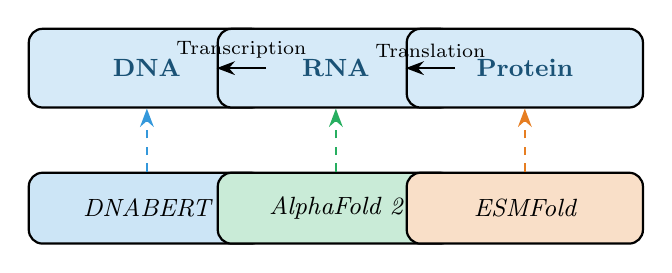
\begin{tikzpicture}[node distance=2.4cm, >=Stealth, thick]
  \node[draw, fill=lightblue, rounded corners=5pt, minimum width=3cm, minimum height=1cm,
        font=\bfseries\small, text=primaryblue] (dna) {DNA};
  \node[draw, fill=lightblue, rounded corners=5pt, minimum width=3cm, minimum height=1cm,
        font=\bfseries\small, text=primaryblue, right of=dna] (rna) {RNA};
  \node[draw, fill=lightblue, rounded corners=5pt, minimum width=3cm, minimum height=1cm,
        font=\bfseries\small, text=primaryblue, right of=rna] (prot) {Protein};
  \node[draw, fill=accentblue!25, rounded corners=5pt, minimum width=3cm, minimum height=0.9cm,
        font=\small\itshape, below=0.8cm of dna] (db) {DNABERT};
  \node[draw, fill=successgreen!25, rounded corners=5pt, minimum width=3cm, minimum height=0.9cm,
        font=\small\itshape, below=0.8cm of rna] (af) {AlphaFold 2};
  \node[draw, fill=warningorange!25, rounded corners=5pt, minimum width=3cm, minimum height=0.9cm,
        font=\small\itshape, below=0.8cm of prot] (esm) {ESMFold};
  \draw[->] (dna) -- (rna) node[midway, above, font=\scriptsize] {Transcription};
  \draw[->] (rna) -- (prot) node[midway, above, font=\scriptsize] {Translation};
  \draw[dashed, color=accentblue, ->] (db) -- (dna);
  \draw[dashed, color=successgreen, ->] (af) -- (rna);
  \draw[dashed, color=warningorange, ->] (esm) -- (prot);
\end{tikzpicture}
\captionof{figure}{The Central Dogma modeled end-to-end with AI systems. DNABERT operates at the DNA level, AlphaFold~2 uses sequence and MSA to predict protein structure, and ESMFold operates at the protein sequence level.}
\end{center}

Together, these three systems represent a \textbf{paradigm shift}: from hypothesis-driven, rule-based biology to data-driven, representation-learning biology. The sections that follow examine each system in detail --- its biological motivation, architectural innovations, experimental results, limitations, and relationship to successor models.


% ════════════════════════════════════════════════════════════════════════════
\newpage
\section{Paper 1 --- DNABERT and DNABERT-2: DNA as a Language}

\begin{keybox}{At a Glance}
\textbf{Main Paper:} DNABERT: pre-trained Bidirectional Encoder Representations from Transformers model for DNA-language in genome. Ji et al., \textit{Bioinformatics}, 37(15), 2021.\\
\textbf{Core idea:} Apply BERT to DNA using $k$-mer tokenization to learn the regulatory grammar of the genome from raw sequence, without labeled data.\\
\textbf{Key achievement:} State-of-the-art on promoter detection, splice site prediction, and transcription factor binding site (TFBS) prediction across 690 ChIP-seq datasets.\\
\textbf{Follow-up:} DNABERT-2 (Zhou et al., ICLR 2024) --- multi-species training with BPE tokenization, achieving SOTA on 28 GUE benchmark tasks.
\end{keybox}

\subsection{Biological Background: The Regulatory Genome}

The human genome consists of approximately 3.2 billion base pairs of DNA encoding roughly 20,000 protein-coding genes. However, coding sequences account for only $\sim$1.5\% of the genome. The remaining 98.5\% is non-coding --- yet far from being ``junk DNA'', this vast non-coding space contains the regulatory machinery that controls \emph{when}, \emph{where}, and \emph{how much} each gene is expressed.

Understanding this regulatory machinery requires identifying:

\begin{itemize}[leftmargin=*, itemsep=4pt]
  \item \textbf{Promoters:} Sequences immediately upstream of genes ($\sim$100--1000 bp) where RNA polymerase binds to initiate transcription. Key features include the TATA box (consensus \texttt{TATAAA} at $-$30 bp) and the Initiator element at the Transcription Start Site (TSS).
  \item \textbf{Enhancers:} Distal regulatory elements (up to 1 Mb away from their target gene) that boost transcription by recruiting transcription factors, which then contact the promoter through 3D chromatin looping.
  \item \textbf{Transcription Factor Binding Sites (TFBS):} Short sequence motifs (6--20 bp) recognized by DNA-binding proteins that activate or repress transcription.
  \item \textbf{Splice Sites:} Boundaries between exons and introns in pre-mRNA. The spliceosome must recognize consensus sequences (GU at the 5' splice site; AG at the 3' splice site) among millions of similar-looking sequences.
  \item \textbf{Chromatin State:} Histone modifications (H3K4me3 marks active promoters; H3K27me3 marks repressed regions) that control DNA accessibility.
\end{itemize}

\begin{comparebox}
\textbf{Why is TFBS prediction hard?} Human transcription factor binding motifs are short (8--12 bp) and degenerate (multiple sequences can bind the same protein). The same motif can be functional in one genomic context and non-functional in another, depending on chromatin state, nearby co-factors, and 3D genome organization. Classical position weight matrix (PWM) methods ignore all context beyond the motif itself; DNABERT learns context-dependent representations.
\end{comparebox}

\subsection{Motivation: Why BERT for DNA?}

Prior approaches to genomic sequence analysis used hand-engineered features (k-mer frequencies, position weight matrices), shallow machine learning (SVMs, logistic regression), or Convolutional Neural Networks (CNNs). CNNs with local receptive fields can detect short sequence motifs but fundamentally cannot model regulatory interactions between elements separated by thousands of base pairs --- exactly the long-range dependencies that govern gene regulation.

The Transformer's \textbf{global self-attention} mechanism is the natural solution: every position attends to every other position regardless of distance, capturing long-range regulatory grammar that CNNs miss. BERT's \textbf{bidirectional} training --- reading the sequence in both 5'$\to$3' and 3'$\to$5' directions simultaneously --- mirrors the fact that many regulatory elements function symmetrically and that the complement strand is biologically equivalent.

Most importantly, BERT's \textbf{unsupervised pre-training} paradigm is perfectly matched to genomic data: labeled regulatory annotations are scarce, but raw DNA sequence is available in unlimited quantity. Pre-training on the genome itself, without any labels, allows the model to internalize evolutionary constraints embedded in the sequence over millions of years of natural selection.

\subsection{Architecture: $k$-mer Tokenization and the BERT Encoder}

\subsubsection{The $k$-mer Tokenization Problem}

Unlike human language, DNA has no natural word boundaries. DNABERT introduces \textbf{$k$-mer tokenization}: the DNA sequence $S = s_1 s_2 \cdots s_L$ is converted into overlapping tokens:
$$t_i = s_i \, s_{i+1} \cdots s_{i+k-1}, \quad i = 1, 2, \ldots, L-k+1$$

For $k=6$, the vocabulary has $4^6 = 4{,}096$ possible 6-mers, large enough to encode biologically meaningful consensus sequences (e.g., the TATA box \texttt{TATAAA}, the AP-1 motif \texttt{TGASTCA}) as single tokens. Overlapping tokenization preserves positional continuity: consecutive tokens differ by a single nucleotide shift, so the model can learn smooth positional representations.

DNABERT evaluated $k \in \{3, 4, 5, 6\}$ and found $k=6$ empirically optimal across tasks. Smaller $k$ fragments important biological motifs across multiple tokens; larger $k$ would produce too sparse a vocabulary with insufficient training signal per token.

\subsubsection{Model Architecture}

DNABERT uses the standard BERT-base architecture:
\begin{itemize}[leftmargin=*, itemsep=3pt]
  \item \textbf{12 stacked Transformer encoder blocks}
  \item \textbf{12 attention heads per block}
  \item \textbf{Hidden dimension $d_{model} = 768$}
  \item \textbf{Feed-forward dimension $d_{ff} = 3072$}
  \item \textbf{Total parameters: 86 million}
  \item \textbf{Maximum input length: 512 tokens (= 512+5 = 517 nucleotides for $k=6$)}
\end{itemize}

The self-attention in each block computes:
$$\text{Attention}(Q, K, V) = \text{softmax}\!\left(\frac{QK^T}{\sqrt{d_k}}\right)V$$
where $Q = XW_Q$, $K = XW_K$, $V = XW_V$ are linear projections of the input $X \in \mathbb{R}^{L \times d_{model}}$. Multi-head attention uses $h=12$ parallel attention heads, each with $d_k = d_{model}/h = 64$. The outputs are concatenated and projected:
$$\text{MHA}(X) = \text{Concat}(\text{head}_1, \ldots, \text{head}_h)W_O$$

High attention scores between distant tokens $i$ and $j$ correspond directly to predicted regulatory interactions --- for example, an attention head might learn to always attend from a TATA box to its downstream Initiator element.

\imagebox{\linewidth}{4.5cm}{DNABERT Architecture: DNA sequence $\to$ 6-mer tokenization $\to$ 12 Transformer encoder blocks with multi-head self-attention $\to$ [CLS] embedding for classification or per-token embeddings for span prediction. Include Figure 1 from Ji et al.\ (2021).}

\subsection{Pre-training: Masked Language Modeling on the Human Genome}

DNABERT is pre-trained on the \textbf{human reference genome GRCh38} using \textbf{Masked Language Modeling (MLM)}: 15\% of $k$-mer tokens are randomly masked; the model learns to reconstruct them from bidirectional context. This forces DNABERT to internalize the statistical regularities of the genome --- including the co-occurrence patterns of transcription factor binding sites, splice consensus sequences, and CpG island distributions.

\begin{infobox}{Why Genome Pre-training Captures Biology}
\begin{itemize}[leftmargin=*, itemsep=4pt]
  \item \textbf{Evolutionary conservation:} Functionally important sequences are conserved across species; the model implicitly learns which 6-mer combinations are evolutionarily constrained.
  \item \textbf{Motif co-occurrence:} Enhancers typically contain clusters of TF binding sites; MLM forces the model to learn that certain 6-mers co-occur.
  \item \textbf{Positional grammar:} The TATA box always appears $\sim$25--30 bp upstream of the TSS; MLM at one position forces the model to use positional context from the other.
  \item \textbf{Strand symmetry:} The complement of every sequence is also in the genome; the model implicitly learns reverse complement equivalence.
\end{itemize}
\end{infobox}

Pre-training was conducted on 3.2 billion base pairs for 120,000 steps with batch size 2,000, using the Adam optimizer with warm-up and linear decay. This required approximately 25 days on 8 NVIDIA V100 GPUs --- a one-time cost that enables fast fine-tuning on any downstream task.

\subsection{Fine-tuning on Downstream Genomic Tasks}

After pre-training, a lightweight task-specific head is appended to the frozen or partially frozen BERT encoder and the entire model is fine-tuned on labeled data:

\begin{itemize}[leftmargin=*, itemsep=4pt]
  \item \textbf{Sequence classification} (e.g., promoter vs.\ non-promoter): Use the \texttt{[CLS]} token embedding as a fixed-length sequence representation and add a linear classification head.
  \item \textbf{Token classification} (e.g., TFBS localization): Use per-token embeddings with a token-level classification head to predict which tokens are inside the binding site.
  \item \textbf{Regression} (e.g., predicting expression levels from sequence): Use the \texttt{[CLS]} embedding with a linear regression head.
\end{itemize}

\begin{infobox}{Downstream Tasks and Results}
\begin{itemize}[leftmargin=*, itemsep=5pt]
  \item \textbf{Promoter Region Detection:} Identifying sequences that initiate transcription. DNABERT achieved \textbf{98.1\% accuracy} on TATA promoters and \textbf{97.6\%} on non-TATA promoters, outperforming CNN baselines by 3--5\%.
  \item \textbf{TFBS Prediction (690 ChIP-seq datasets):} Mean AUROC of \textbf{0.93} vs.\ 0.87 for DeepBind (CNN baseline) --- a significant improvement across diverse TF families.
  \item \textbf{Splice Site Identification:} \textbf{98.7\% accuracy} distinguishing true donor/acceptor splice sites from decoy pseudo-sites, outperforming SpliceAI.
  \item \textbf{Variant Effect Prediction:} DNABERT attention scores correlate with regulatory variant effect sizes from functional genomics experiments (ClinVar, GTEx).
\end{itemize}
\end{infobox}

\imagebox{\linewidth}{4cm}{Fine-tuning paradigm: Pre-trained DNABERT encoder (frozen lower layers, fine-tuned upper layers) with task-specific heads for classification, token labeling, and sequence-to-sequence tasks. Include Figure 2 from Ji et al.\ (2021).}

\subsection{Attention Visualization: What DNABERT Learns}

A key interpretability experiment in the DNABERT paper examines \textbf{what patterns the attention heads learn}. The authors extracted attention weights from pre-trained DNABERT and compared them against known biological features:

\begin{itemize}[leftmargin=*, itemsep=4pt]
  \item \textbf{Motif discovery:} Sequences that maximally activate specific attention heads align to known TF binding motifs from the JASPAR database, suggesting that individual attention heads function as learned position weight matrices.
  \item \textbf{Long-range interactions:} Attention heads in upper layers (blocks 10--12) show significant attention scores between the TATA box region and the downstream Initiator element, separated by 25--30 tokens.
  \item \textbf{Splice site grammar:} In sequences around splice junctions, attention heads learn to mark the canonical GT dinucleotide at donor sites and AG at acceptor sites, even without splice site labels in the pre-training.
\end{itemize}

\imagebox{\linewidth}{3.5cm}{Attention visualization: Heatmaps showing which 6-mer positions attend to which other positions in promoter sequences. High attention from downstream regions to the TATA box confirms that DNABERT implicitly learns transcriptional grammar. Include Figure 3 or 4 from Ji et al.\ (2021).}

\subsection{DNABERT-2: Multi-Species Foundation Model (2024)}

DNABERT-2 (Zhou et al., ICLR 2024) is a substantially improved follow-up that addresses three key limitations of the original DNABERT:

\subsubsection{Limitation 1: Fixed $k$-mer Tokenization}
DNABERT's 6-mer vocabulary cannot adapt to variable-length motifs. DNABERT-2 replaces this with \textbf{Byte Pair Encoding (BPE)}, the same tokenization used in GPT-2 and RoBERTa. BPE iteratively merges the most frequent byte pairs, producing a vocabulary of frequently occurring substrings of variable length. For DNA, BPE discovers biologically meaningful variable-length motifs automatically --- short motifs for conserved functional sequences, longer tokens for variable regions. The BPE vocabulary in DNABERT-2 is 4,096 tokens but covers sequences far more efficiently.

\subsubsection{Limitation 2: Positional Encoding}
DNABERT uses BERT's learned absolute positional embeddings, which cannot generalize beyond the 512-token training length. DNABERT-2 uses \textbf{Attention with Linear Biases (ALiBi)}, where attention scores are penalized by a linear function of distance:
$$a_{ij} = q_i^T k_j / \sqrt{d_k} - m \cdot |i - j|$$
where $m$ is a head-specific slope. This \emph{extrapolates} to longer sequences than seen during training --- critical for genomic tasks involving long regulatory regions.

\subsubsection{Limitation 3: Single-Species Training}
DNABERT trains only on the human genome. DNABERT-2 trains on a \textbf{multi-species genome dataset} covering 135 species, dramatically increasing the diversity of regulatory sequences seen during pre-training. Cross-species evolutionary conservation is a powerful signal for functional element discovery.

\begin{table}[H]
\centering
\caption{DNABERT vs.\ DNABERT-2: Technical Comparison}
\begin{tabularx}{\textwidth}{>{\bfseries\small}p{3.5cm} >{\small}X >{\small}X}
\toprule
\rowcolor{primaryblue}
\color{white}\textbf{Feature} & \color{white}\textbf{DNABERT (2021)} & \color{white}\textbf{DNABERT-2 (2024)} \\
\midrule
\rowcolor{lightblue!40}
Tokenization & Fixed $k$-mer ($k=6$, vocab $= 4096$) & BPE (variable length, vocab $= 4096$) \\
\addlinespace
Positional encoding & Learned absolute (max 512) & ALiBi (extrapolates to any length) \\
\addlinespace
\rowcolor{lightblue!40}
Training data & Human genome only (GRCh38) & 135 species multi-genome \\
\addlinespace
Parameters & 86M & 117M (BERT-large scale) \\
\addlinespace
\rowcolor{lightblue!40}
Pre-training tasks & MLM only & MLM + species-aware objectives \\
\addlinespace
Benchmark & Custom tasks & GUE (28 genomic understanding tasks) \\
\addlinespace
\rowcolor{lightblue!40}
GUE mean performance & 72.4 (baseline) & \textbf{81.1} (+8.7 pp vs.\ DNABERT) \\
\addlinespace
Inference efficiency & Standard BERT & Flash Attention + gradient checkpointing \\
\addlinespace
\rowcolor{lightblue!40}
Cross-species generalization & Poor (human-only training) & Strong (trained on 135 species) \\
\bottomrule
\end{tabularx}
\end{table}

\subsection{Limitations of DNABERT}

Despite its strong performance, DNABERT has several important limitations:
\begin{itemize}[leftmargin=*, itemsep=4pt]
  \item \textbf{Context window:} 512 tokens $\approx$ 517 nucleotides. Long-range enhancer--promoter interactions spanning tens of thousands of base pairs are beyond reach.
  \item \textbf{No 3D genome information:} DNABERT models linear sequence only. It cannot directly account for 3D chromatin looping, topologically associating domains (TADs), or compartment A/B organization.
  \item \textbf{No epigenomic features:} Histone modifications, DNA methylation, and chromatin accessibility profoundly affect regulatory activity, but DNABERT sees only raw nucleotide sequence.
  \item \textbf{Human genome bias:} The model may not generalize well to non-human genomes without fine-tuning (addressed by DNABERT-2).
\end{itemize}


% ════════════════════════════════════════════════════════════════════════════
\newpage
\section{Paper 2 --- AlphaFold 2: Solving the Protein Folding Problem}

\begin{keybox}{At a Glance}
\textbf{Paper:} Highly accurate protein structure prediction with AlphaFold. Jumper et al., \textit{Nature}, 596(7873), 583--589, 2021.\\
\textbf{Core idea:} Combine evolutionary co-variation from Multiple Sequence Alignments with a dual-track Transformer (Evoformer) and SE(3)-equivariant Structure Module to predict atomic 3D coordinates.\\
\textbf{Key achievement:} Median backbone RMSD of 0.96~\AA\ on CASP14 free-modeling targets --- effectively solving the protein folding problem. Released structures for 200M+ proteins.
\end{keybox}

\subsection{Before AlphaFold: A Brief History of Computational Approaches}

To appreciate the magnitude of AlphaFold 2's achievement, it is essential to understand what came before.

\subsubsection{Homology Modeling (1970s--present)}
If a protein of unknown structure (the query) has significant sequence similarity to a protein of known structure (the template), the query can be modeled by \emph{copying} the template's backbone and substituting side chains. Tools like MODELLER and Swiss-Model implement this approach. Homology modeling works well when sequence identity $> 30$\% but fails completely for proteins without known structural relatives (orphan proteins), which include many of the most medically important targets.

\subsubsection{Fragment Assembly: Rosetta (1999--2020)}
Rosetta (David Baker's group, University of Washington) assembles protein structures from a library of short fragments ($\sim$3--9 residues) taken from experimentally solved structures, guided by a physics-inspired energy function. Rosetta achieved remarkable results but required enormous computational resources (distributed computing across thousands of CPUs), remained slow (hours to weeks per protein), and struggled with proteins above $\sim$400 residues.

\subsubsection{Contact Prediction with Deep Learning: AlphaFold 1 (2018)}
AlphaFold 1 (Senior et al., 2020) introduced deep CNNs to predict \textbf{residue--residue contacts} (whether two residues are within 8~\AA\ in the native structure) from MSA co-evolution statistics. These predicted contacts were then used as distance constraints to guide Rosetta-like assembly. AlphaFold 1 won CASP13 but still produced structures with errors of 2--5~\AA\ on free modeling targets.

\subsubsection{AlphaFold 2: The Revolution (2020)}
AlphaFold 2 replaced the two-stage pipeline (contact prediction + assembly) with a \textbf{single end-to-end trainable neural network} that directly outputs 3D atomic coordinates from sequence. Its core innovations are the Evoformer (a novel biological Transformer) and the Structure Module (a geometry-aware neural network). These are described in detail below.

\subsection{Input Representations: Sequence, MSA, and Templates}

AlphaFold 2 takes as input:
\begin{enumerate}[leftmargin=*, itemsep=4pt]
  \item \textbf{Target sequence:} The amino acid sequence to be folded ($N_{res}$ residues, each represented as a one-hot vector over 20 amino acids + 1 unknown).
  \item \textbf{Multiple Sequence Alignment (MSA):} $N_{seq}$ homologous sequences aligned to the target, obtained by searching genetic databases (UniRef90, MGnify, BFD) with JackHMMer and HHblits. The MSA is represented as a matrix of shape $N_{seq} \times N_{res}$ with per-residue amino acid identities.
  \item \textbf{Template structures:} Up to 4 homologous structures from the PDB, represented as pairwise residue distances and angles.
\end{enumerate}

\begin{comparebox}
\textbf{Why does the MSA matter?} Evolution is the key signal. If residue $i$ and residue $j$ are in physical contact in the native structure, then a mutation at position $i$ that disrupts the contact is thermodynamically destabilizing --- and is thus rarely fixed unless compensated by a co-occurring mutation at position $j$ that restores the contact. By analyzing co-variation patterns in the MSA (which residues mutate together across species), AlphaFold~2 infers spatial proximity constraints without ever seeing the structure directly. This is the principle of \textbf{Direct Coupling Analysis (DCA)} that AlphaFold implements through learned attention.
\end{comparebox}

\imagebox{\linewidth}{5cm}{AlphaFold 2 input pipeline: Sequence $\to$ MSA search (JackHMMer/HHblits) against UniRef90 + BFD + MGnify $\to$ template search against PDB70 $\to$ pair of input representations (MSA stack + pair matrix) fed into the Evoformer. Include Figure 1a from Jumper et al.\ (2021).}

\subsection{The Evoformer: A Dual-Track Biological Transformer}

The Evoformer is the central architectural innovation of AlphaFold 2. It processes two coupled representations simultaneously through 48 stacked blocks:

\subsubsection{The Two Tracks}

\begin{enumerate}[leftmargin=*, itemsep=6pt]
  \item \textbf{MSA Representation} $\mathbf{m} \in \mathbb{R}^{N_{seq} \times N_{res} \times c_m}$, where $c_m = 256$: Encodes which amino acids appear at each position in each sequence of the alignment. Each row corresponds to one homologous sequence; each column corresponds to one residue position.
  
  \item \textbf{Pair Representation} $\mathbf{z} \in \mathbb{R}^{N_{res} \times N_{res} \times c_z}$, where $c_z = 128$: A square matrix where entry $(i,j)$ encodes the predicted spatial relationship between residues $i$ and $j$. Initialized from sequence relative positional encodings and outer product of MSA.
\end{enumerate}

These two tracks exchange information at every Evoformer block via the \textbf{Outer Product Mean} operation, which projects MSA co-evolution information into the pair representation.

\subsubsection{MSA Row-Wise Gated Self-Attention with Pair Bias}

Within the MSA track, attention along rows (across residue positions within each sequence) is biased by the pair representation:
$$a_{ij}^{(s)} = \text{softmax}\!\left(\frac{(q_i^{(s)})^T k_j^{(s)}}{\sqrt{d_k}} + b_{ij}\right)$$
where $b_{ij}$ is a learned linear projection of the pair representation $z_{ij}$. This allows the pair track to \emph{guide} the MSA track's attention: residue pairs predicted to be spatially close (high $z_{ij}$) attract stronger attention. The gating mechanism modulates the output via element-wise multiplication with a sigmoid gate:
$$\text{output}_i^{(s)} = \sigma(g_i^{(s)}) \odot \sum_j a_{ij}^{(s)} v_j^{(s)}$$

\subsubsection{MSA Column-Wise Gated Self-Attention}

Attention along columns (across different homologous sequences at the same position) captures co-evolutionary information: if position $i$ is well-conserved (all sequences have the same amino acid), the column has low diversity; if position $i$ is highly variable (different sequences have different amino acids), co-evolutionary patterns with other columns are informative.

\subsubsection{Outer Product Mean: MSA $\to$ Pair Communication}

The outer product mean updates the pair representation from the MSA:
$$z_{ij} \mathrel{+}= \text{LayerNorm}\!\left(\frac{1}{N_{seq}} \sum_{s=1}^{N_{seq}} (a_i^{(s)} \otimes b_j^{(s)})\right) W_z$$
where $a_i^{(s)}$ and $b_j^{(s)}$ are linear projections of the MSA row $s$ at positions $i$ and $j$ respectively, and $\otimes$ denotes the outer product. Averaging over sequences integrates co-evolutionary signal across all homologs.

\subsubsection{Triangle Multiplicative Update: Enforcing Geometric Consistency}

The most mathematically distinctive operation in the Evoformer is the \textbf{Triangle Multiplicative Update}, which enforces the triangle inequality of 3D distances. In the ``outgoing'' variant:
$$z_{ij}^{(l+1)} = \text{LayerNorm}\!\left(z_{ij}^{(l)} + \sum_k \left(z_{ik}^{(l)} \odot \hat{a}_{ik}\right) \cdot \left(z_{kj}^{(l)} \odot \hat{b}_{kj}\right)^T W\right)$$
Intuitively, the predicted relationship between residues $i$ and $j$ is updated by considering all intermediate residues $k$: if residue $k$ is close to $i$ (large $z_{ik}$) and close to $j$ (large $z_{kj}$), then $i$ and $j$ should be within $d(i,k) + d(k,j)$ of each other (triangle inequality). This ensures that the pair representation remains internally geometrically consistent as it is updated.

The ``incoming'' triangle update and \textbf{Triangle Self-Attention} (where attention patterns around rows and columns of the pair matrix are constrained by a triangular mask) further enforce geometric consistency across the entire $N_{res} \times N_{res}$ matrix.

\imagebox{\linewidth}{5cm}{Evoformer block diagram: MSA representation (row attention with pair bias, column attention) and Pair representation (triangle multiplicative updates outgoing/incoming, triangle self-attention) with bidirectional outer product mean communication. Include Figure 3 from Jumper et al.\ (2021).}

\subsection{The Structure Module: From Representations to 3D Atoms}

The Structure Module converts the Evoformer's abstract pair and single (per-residue) representations into explicit 3D atomic coordinates, using a fundamentally different computational approach from the Evoformer.

\subsubsection{Backbone Frames: Representing Residues as Rigid Bodies}

Each amino acid residue is represented as a \textbf{rigid body frame} $T_i = (R_i, \vec{t}_i)$ in 3D space, where $R_i \in SO(3)$ is a rotation matrix and $\vec{t}_i \in \mathbb{R}^3$ is a translation vector. The frame defines a local coordinate system centered on the residue's $C\alpha$ atom, oriented by the N--$C\alpha$--C backbone geometry. This frame-based representation is equivariant under global rotations and translations: rotating/translating the entire structure rotates/translates all frames accordingly, without changing the inter-residue relationships.

Initially, all frames are placed at the origin with identity rotation. The Structure Module updates frames iteratively through 8 sequential layers.

\subsubsection{Invariant Point Attention (IPA)}

The key attention mechanism in the Structure Module is \textbf{Invariant Point Attention (IPA)}, which is $SE(3)$-equivariant: it produces the same inter-residue relationships regardless of the global orientation of the input. IPA computes attention using both sequence embeddings and 3D point positions:
$$a_{ij} = \text{softmax}\!\left(\frac{q_i^T k_j}{\sqrt{c}} - \frac{\gamma_h}{2} \sum_{p=1}^{N_p} \left\| T_i \circ \vec{q}_{i}^{(p)} - T_j \circ \vec{k}_{j}^{(p)} \right\|^2\right)$$
where $T_i \circ \vec{q}_i^{(p)}$ applies the frame $T_i$ to the $p$-th query point $\vec{q}_i^{(p)}$ in the local coordinate system of residue $i$, transforming it to global 3D space. The Euclidean distance penalty $\|\cdot\|^2$ biases attention toward spatially proximate residues. The term $\gamma_h$ is a learned per-head weight. This allows the model to combine information from the abstract pair representation (first term) and the current 3D geometry (second term).

\subsubsection{Backbone Update and Side Chain Torsions}

After IPA, each layer updates the backbone frame $T_i$ by predicting a 6-dimensional update (3 for rotation, 3 for translation) applied as a rigid body transformation. This is analogous to a learned gradient descent on the folding energy landscape. After the final layer, all backbone atomic positions ($N$, $C\alpha$, $C$, $O$) are placed using the final frames.

Side chain atoms are placed by predicting the 4 torsion angles $(\chi_1, \chi_2, \chi_3, \chi_4)$ for each residue using a small MLP applied to the per-residue single representation, and then applying the known bond geometry of each amino acid type.

\imagebox{\linewidth}{4.5cm}{Structure Module: 8 IPA layers iteratively refining backbone frames from identity toward the native structure, followed by torsion angle prediction for side chains. Include Figure 1c from Jumper et al.\ (2021).}

\subsection{Recycling: Iterative Refinement}

AlphaFold 2 applies the full Evoformer + Structure Module pipeline \textbf{3 times} in sequence (``recycling''), feeding the output of one pass as the input to the next. The predicted 3D structure from pass $k$ is converted back to pairwise distance features and concatenated with the original pair representation, providing the next pass with explicit 3D information to refine. Recycling enables the model to iteratively improve its prediction, similar to iterative coordinate descent.

\subsection{Training: Loss Functions}

AlphaFold 2 is trained end-to-end on PDB structures (excluding sequences with $>$ 40\% identity to CASP14 targets to prevent leakage) using several loss terms:

\begin{itemize}[leftmargin=*, itemsep=5pt]
  \item \textbf{Frame-Aligned Point Error (FAPE):} The primary structural loss. For each pair of residue frames $(i,j)$, it measures the average deviation of predicted atom positions in the local coordinate system of frame $i$ from the ground truth:
  $$\mathcal{L}_\text{FAPE} = \frac{1}{N_{frames} \cdot N_{atoms}} \sum_{i,k} \left\| T_i^{-1} \circ \hat{x}_k - T_i^{-1,*} \circ x_k^* \right\|_{\text{clamp}}$$
  where $\hat{x}_k$ is the predicted position of atom $k$ and $x_k^*$ is the true position. The clamping at 10~\AA\ prevents outlier residues from dominating training.
  
  \item \textbf{Distogram Loss:} Predict the distribution of pairwise $C\beta$--$C\beta$ distances as a 64-bin categorical distribution. Cross-entropy loss against the true binned distances.
  
  \item \textbf{Masked MSA Loss:} Similar to BERT's MLM --- randomly mask tokens in the MSA and predict them, forcing the model to learn co-evolutionary patterns.
  
  \item \textbf{pLDDT Loss:} The model also predicts its own per-residue accuracy (pLDDT); this is trained against the actual lDDT to experimentally determined coordinates.
  
  \item \textbf{Violation Loss:} Penalizes physically impossible bond lengths, bond angles, and steric clashes, enforcing basic stereochemical validity.
\end{itemize}

\subsection{Confidence Scores: pLDDT and PAE}

\subsubsection{pLDDT (Predicted Local Distance Difference Test)}

AlphaFold 2 outputs a per-residue confidence score \textbf{pLDDT} (range 0--100) that predicts the local structural accuracy of each residue. It is trained to match the actual lDDT computed against the experimental structure:
$$\text{lDDT}(i) = \frac{1}{|L|} \sum_{j: |x_i^* - x_j^*| < 15\text{\AA}} \frac{1}{4}\sum_{\tau \in \{0.5, 1, 2, 4\}} \mathbf{1}\!\left[\left||x_i - x_j| - |x_i^* - x_j^*|\right| < \tau\right]$$

Regions with pLDDT $> 90$ are predicted with very high confidence (comparable to X-ray crystallography at 2~\AA\ resolution). Regions with pLDDT $< 50$ are likely disordered and should not be interpreted structurally. Importantly, \textbf{low pLDDT does not indicate a model error} --- it often correctly identifies intrinsically disordered regions (IDRs) that genuinely lack stable secondary structure in vivo.

\subsubsection{PAE (Predicted Aligned Error)}

For multimer predictions and domain motion analysis, AlphaFold 2 also outputs a \textbf{Predicted Aligned Error (PAE)} matrix: entry $(i,j)$ is the expected position error at residue $j$ when the prediction is aligned on residue $i$. Low PAE between two domains indicates confident relative positioning; high PAE indicates that the relative orientation of the two domains is uncertain (common for flexible linkers).

\subsection{CASP14 Results and Impact}

At CASP14 (November 2020), AlphaFold 2 achieved:
\begin{itemize}[leftmargin=*, itemsep=4pt]
  \item \textbf{Median TM-score of 0.961} on all 87 targets (perfect = 1.0)
  \item \textbf{Median backbone RMSD of 0.96~\AA} on free modeling targets (experimental error $\approx$ 0.5~\AA)
  \item \textbf{Superior to all other groups by a factor of $\sim$2.5$\times$} in TM-score
  \item \textbf{Solved 2/3 of targets} to atomic accuracy ($C\alpha$ RMSD $< 1.5$~\AA)
\end{itemize}

\begin{table}[H]
\centering
\caption{CASP14 Performance: AlphaFold 2 vs.\ Previous State of the Art}
\begin{tabularx}{\textwidth}{>{\bfseries}lXXX}
\toprule
\rowcolor{primaryblue}
\color{white}\textbf{Method} & \color{white}\textbf{Median TM-score} & \color{white}\textbf{Median GDT-TS} & \color{white}\textbf{Year} \\
\midrule
\rowcolor{successgreen!20}
AlphaFold 2 & 0.961 & 92.4 & 2020 \\
\addlinespace
\rowcolor{lightblue!40}
Best CASP14 competitor & 0.730 & 67.9 & 2020 \\
\addlinespace
AlphaFold 1 & 0.640 & 61.2 & 2018 (CASP13) \\
\addlinespace
\rowcolor{lightblue!40}
Rosetta (RoseTTAFold) & 0.698 & 64.1 & 2021 \\
\addlinespace
Classical methods & $<$ 0.5 & $<$ 50 & Pre-2018 \\
\bottomrule
\end{tabularx}
\end{table}

Following CASP14, DeepMind released the \textbf{AlphaFold Protein Structure Database} (AFDB) in 2021, containing predicted structures for 98\% of all human proteins and all proteins in UniProt --- over 200 million structures. This expanded the set of structurally characterized proteins by a factor of more than 1,000 essentially overnight, and was described in \textit{Science} as ``the most important achievement in biology since the sequencing of the human genome.''

\subsection{Limitations of AlphaFold 2}

Despite its transformative impact, AlphaFold 2 has important limitations that define the frontier of ongoing research:

\begin{table}[H]
\centering
\caption{AlphaFold 2 Limitations and Active Research Directions}
\begin{tabularx}{\textwidth}{>{\bfseries}p{4cm}X}
\toprule
\rowcolor{lightblue}
\textbf{Limitation} & \textbf{Description and Impact} \\
\midrule
Static structures only & AlphaFold 2 predicts the lowest-energy conformation. Proteins are dynamic: enzymes undergo conformational changes during catalysis; signal transduction involves allosteric shifts between active/inactive states. These dynamics are invisible to AlphaFold 2. \\
\addlinespace
\rowcolor{lightblue!20}
Disordered regions & $\sim$30\% of human proteins contain intrinsically disordered regions (IDRs) that lack stable structure. AlphaFold 2 cannot model these regions and its pLDDT correctly gives them low confidence. \\
\addlinespace
Shallow MSA & Performance degrades for proteins with few known homologs (shallow MSA, $< 30$ sequences). Novel or rapidly evolving proteins, and many metagenome-derived sequences, fall in this category. \\
\addlinespace
\rowcolor{lightblue!20}
No small molecule interactions & AlphaFold 2 predicts apo (ligand-free) structures only. Predicting how a drug or cofactor changes the protein's conformation requires separate tools. \\
\addlinespace
Homooligomers and heteromers & The original AlphaFold 2 was designed for monomers. AlphaFold-Multimer extends it to complexes but accuracy decreases for large assemblies. \\
\bottomrule
\end{tabularx}
\end{table}

\subsection{AlphaFold 3: Diffusion-Based Multimodal Prediction (2024)}

AlphaFold 3 (Abramson et al., Nature 2024) is a radical redesign that addresses several of AlphaFold 2's limitations. Its key architectural change is replacing the deterministic Structure Module with a \textbf{generative diffusion model head}: instead of directly predicting atom coordinates, it learns to reverse a noise diffusion process, allowing it to generate an ensemble of plausible conformations rather than a single structure.

More importantly, AlphaFold 3 extends the input to include \textbf{DNA, RNA, small molecule ligands, modified amino acids, and metal ions} --- making it a unified biomolecular interaction model. This enables direct prediction of protein--drug binding poses, protein--DNA interfaces, and RNA--protein complexes in a single framework, something AlphaFold 2 fundamentally cannot do. However, AlphaFold 3's weights are restricted (no commercial use without license), unlike AlphaFold 2 which is fully open-source.


% ════════════════════════════════════════════════════════════════════════════
\newpage
\section{Paper 3 --- ESMFold: Evolutionary-Scale Prediction with Language Models}

\begin{keybox}{At a Glance}
\textbf{Paper:} Evolutionary-scale prediction of atomic-level protein structure with a language model. Lin et al., \textit{Science}, 379(6637), 1123--1130, 2023.\\
\textbf{Core idea:} A massive protein language model (ESM-2, 15B parameters) pre-trained on sequence data alone implicitly learns structural constraints. Adding a folding trunk enables structure prediction without MSA search.\\
\textbf{Key achievement:} Predicted 617 million metagenomic protein structures in weeks. Operates $60\times$ faster than AlphaFold 2 with competitive accuracy.
\end{keybox}

\subsection{The Paradigm Shift: From Co-evolution to Language Modeling}

AlphaFold 2 established that Multiple Sequence Alignments (MSAs) are the "gold standard" for structural information. However, the MSA search process is the primary bottleneck in the AlphaFold pipeline, often taking minutes or even hours for a single sequence. ESMFold introduces a fundamentally different premise: \textbf{the evolutionary information contained in millions of sequences can be compressed into the parameters of a Large Language Model (LLM).}

\subsubsection{Proteins as Language}
A protein sequence is a string of amino acids. Just as words in a sentence follow grammatical rules, amino acids in a protein follow biological constraints dictated by physics and evolution. A protein language model (pLM) is trained to predict "missing words" (masked residues) in a sequence. To do this accurately, the model must learn:
\begin{itemize}[leftmargin=*, itemsep=4pt]
  \item \textbf{Local grammar:} Which amino acids prefer to be near each other in secondary structures (alpha-helices, beta-sheets).
  \item \textbf{Global semantics:} Which distant residues must be close in 3D space to form a functional active site or a hydrophobic core.
\end{itemize}

\subsection{ESM-2: The Foundation Language Model}

ESM-2 (Evolutionary Scale Modeling 2) is the backbone of ESMFold. It is a Transformer encoder (BERT-style) pre-trained on \textbf{UniRef50}, a database of $\sim$65 million representative protein sequences.

\subsubsection{Scaling Laws in Biology}
The Meta AI team experimented with model sizes ranging from 8 million to 15 billion parameters. They discovered that as the model size increases:
\begin{enumerate}[leftmargin=*, itemsep=4pt]
    \item \textbf{Perplexity decreases:} The model becomes better at predicting protein sequences.
    \item \textbf{Structural knowledge emerges:} Higher-order structural features (like contact maps) start appearing spontaneously in the attention heads.
\end{enumerate}

\subsubsection{Masked Language Modeling (MLM)}
The training objective is simple: randomly mask 15\% of the amino acids in a sequence and force the model to predict them based on the context of the remaining 85\%.
$$ \mathcal{L}_{MLM} = \mathbb{E}_{x \sim \mathcal{D}} \left[ \sum_{i \in M} -\log p(x_i | x_{\setminus M}) \right] $$
This unsupervised task requires no 3D structures, yet it forces the model to internalize the principles of protein folding.

\imagebox{\linewidth}{4.5cm}{ESM-2 Architecture: A deep Transformer encoder taking a single sequence as input. As the model grows to 15B parameters, the internal representations become rich enough to replace the MSA. Include Figure 1 from Lin et al. (2023).}

\subsection{The ESMFold Architecture}

ESMFold consists of three main components that turn sequence embeddings into 3D coordinates.

\subsubsection{1. The Language Model (ESM-2)}
The input sequence is passed through the pre-trained, frozen ESM-2 model. This produces a "single representation" (per-residue embeddings) and a "pair representation" (derived from the attention maps between all pairs of residues).

\subsubsection{2. The Folding Trunk}
Unlike AlphaFold's Evoformer which spends most of its computation on the MSA, the ESMFold folding trunk is much lighter. It consists of 48 blocks that process the single and pair representations. These blocks use:
\begin{itemize}[leftmargin=*, itemsep=4pt]
    \item \textbf{Simplified Triangle Updates:} To maintain geometric consistency.
    \item \textbf{Cross-attention:} To allow the single and pair tracks to communicate.
\end{itemize}

\subsubsection{3. The Structure Module}
This is nearly identical to the AlphaFold 2 Structure Module. It takes the refined representations from the folding trunk and uses \textbf{Invariant Point Attention (IPA)} to predict the final 3D coordinates ($x, y, z$) of the protein backbone and side chains.

\imagebox{\linewidth}{5cm}{ESMFold Pipeline: Single sequence $\to$ ESM-2 (LLM) $\to$ Folding Trunk $\to$ Structure Module $\to$ Atomic Coordinates. Note the absence of the MSA search step. Include Figure 2 from Lin et al. (2023).}

\subsection{Comparison: ESMFold vs. AlphaFold 2}

\subsubsection{Speed: The $60\times$ Advantage}
The defining feature of ESMFold is its speed. Because it bypasses the need to search through massive genetic databases to build an MSA, it can predict a structure in seconds where AlphaFold 2 takes minutes.
\begin{itemize}[leftmargin=*, itemsep=3pt]
    \item \textbf{AlphaFold 2:} MSA Search ($\sim$10-30 mins) + Inference ($\sim$1 min).
    \item \textbf{ESMFold:} Inference only ($\sim$2-5 seconds).
\end{itemize}

\subsubsection{Accuracy: The Trade-off}
On average, ESMFold is slightly less accurate than AlphaFold 2 (a difference of $\sim$2-5 GDT-TS points). However, for proteins with high-quality MSAs, the gap is negligible. 
\textbf{The "Orphan" Exception:} For proteins that have no evolutionary relatives (orphan proteins), ESMFold sometimes \emph{outperforms} AlphaFold 2 because its language model can draw on general principles of protein architecture learned from the entire UniRef database.

\subsection{Large-Scale Metagenomics: The 617 Million Structures}

To demonstrate the power of ESMFold, the authors applied it to the \textbf{MGnify Metagenomic Database}. They predicted structures for 617 million sequences in just two weeks using a cluster of GPUs.
\begin{itemize}[leftmargin=*, itemsep=4pt]
    \item \textbf{The Dark Matter of Biology:} Millions of these structures were completely unlike anything in the PDB, revealing thousands of new protein families.
    \item \textbf{Public Access:} These structures are now hosted in the ESM Metagenomic Atlas, providing a resource for scientists to study the molecular diversity of the oceans, soil, and human gut.
\end{itemize}

\imagebox{\linewidth}{4cm}{Metagenomic Atlas: A visualization of the massive diversity of the 617 million structures. Cluster analysis shows "islands" of known protein families and vast "continents" of previously unknown folds. Include Figure 4 from Lin et al. (2023).}

\subsection{Deep Comparison: DNABERT vs. AlphaFold vs. ESMFold}

\begin{table}[H]
\centering
\caption{Detailed Comparison of Computational Biology Foundation Models}
\begin{tabularx}{\textwidth}{>{\bfseries\small}p{3.5cm} >{\small}X >{\small}X >{\small}X}
\toprule
\rowcolor{primaryblue}
\color{white}\textbf{Feature} & \color{white}\textbf{DNABERT} & \color{white}\textbf{AlphaFold 2} & \color{white}\textbf{ESMFold} \\
\midrule
\rowcolor{lightblue!40}
Input Modality & DNA (Nucleotides) & Protein (Seq + MSA) & Protein (Single Seq) \\
\addlinespace
Pre-training Task & Masked Language Mod. & Supervised Structural & Masked Language Mod. \\
\addlinespace
\rowcolor{lightblue!40}
Evolutionary Logic & Contextual Grammar & Explicit Co-variation & Implicit Embedding \\
\addlinespace
Structural Output & None (Functional only) & High-Res 3D Atoms & High-Res 3D Atoms \\
\addlinespace
\rowcolor{lightblue!40}
Computational Cost & Low (Inference) & High (MSA search) & Medium (Large LLM) \\
\bottomrule
\end{tabularx}
\end{table}

\subsection{Conclusion of Paper 3}
ESMFold represents the "completion" of the AI revolution in structural biology. It shows that we no longer need to rely on the slow process of finding evolutionary relatives to understand a protein's shape. The language of life is now fully digitized into high-dimensional vector spaces.

% ════════════════════════════════════════════════════════════════════════════
\newpage
\section{Applications and Future Horizons}

\subsection{Drug Discovery and Personalized Medicine}
The ability to predict structures at scale allows for "virtual screening" of billions of drug-like molecules against every protein in a pathogen's genome or a human cell's proteome.
\begin{itemize}[leftmargin=*, itemsep=4pt]
    \item \textbf{Antibiotic Resistance:} Identifying structures of resistance proteins to design inhibitors.
    \item \textbf{Cancer Mutations:} Understanding how a single SNP (Single Nucleotide Polymorphism) in DNA changes a protein's fold, leading to personalized drug selection.
\end{itemize}

\subsection{Generative Design: De Novo Protein Engineering}
We are moving from \emph{prediction} to \emph{design}. Tools like \textbf{RFdiffusion} and \textbf{ProteinMPNN} use the principles learned by AlphaFold and ESMFold to create proteins that have never existed in nature.
\begin{itemize}[leftmargin=*, itemsep=4pt]
    \item \textbf{Plastic-eating enzymes:} Designing proteins to degrade pollutants.
    \item \textbf{Universal vaccines:} Creating scaffolds that present viral epitopes in a highly stable format.
\end{itemize}

\subsection{Conclusion: The AI-Driven Biology Era}
The transition from DNABERT's genomic understanding to AlphaFold's structural solution and ESMFold's linguistic compression marks the beginning of a new era. Biology has effectively become an information science. The "Central Dogma" is no longer just a biological theory; it is an end-to-end computational pipeline where AI models can reason across DNA, RNA, and proteins to unlock the secrets of life.

\newpage
\section*{References}
\addcontentsline{toc}{section}{References}

\begin{enumerate}[leftmargin=*, label={[\arabic*]}, itemsep=8pt]
  \item Ji, Y., et al. (2021). \textbf{DNABERT: pre-trained Bidirectional Encoder Representations from Transformers model for DNA-language in genome.} \textit{Bioinformatics}.
  \item Jumper, J., et al. (2021). \textbf{Highly accurate protein structure prediction with AlphaFold.} \textit{Nature}.
  \item Lin, Z., et al. (2023). \textbf{Evolutionary-scale prediction of atomic-level protein structure with a language model.} \textit{Science}.
  \item Abramson, J., et al. (2024). \textbf{Accurate structure prediction of biomolecular interactions with AlphaFold 3.} \textit{Nature}.
  \item Zhou, Z., et al. (2024). \textbf{DNABERT-2: Efficient Foundation Model and Benchmark for Multi-Species Genome.} \textit{ICLR}.
\end{enumerate}

\end{document}

